\documentclass{beamer}
\usepackage{graphicx} % Required for inserting images
\usepackage{caption}
\newcommand{\source}[1]{\caption*{Source: {#1}} }
\usepackage{pifont}

\usepackage{tikz}
\title[]{Secure Streaming with Fog Offloading}


\author[Oliveira, Joaquim]
{By Joaquim Tiago Gonçalves Oliveira\inst{1} \\ Supervisor Rolando Martins\inst{1}}

\date[Nov. 2025]
{November, 2025}

\institute[FCUP]
{
  \inst{1}%
  Department of Computer Science\\
  Faculty of Science of the University of Porto
}

\logo{
\includegraphics[height=0.5cm]{fcup-identidade-logotipo-cores.png}}

\usetheme{Madrid}
\usecolortheme{default}

\setbeamertemplate{footline}{%
  \leavevmode%
  \hbox{%
    \begin{beamercolorbox}[wd=.33\paperwidth,ht=2.5ex,dp=1ex,left]{author in head/foot}%
      \hspace*{2mm}\insertshortauthor, \insertshortinstitute, \insertshortdate
    \end{beamercolorbox}%
    \begin{beamercolorbox}[wd=.34\paperwidth,ht=2.5ex,dp=1ex,center]{title in head/foot}%
      \insertshorttitle
    \end{beamercolorbox}%
    \begin{beamercolorbox}[wd=.33\paperwidth,ht=2.5ex,dp=1ex,right]{section in head/foot}%
      \insertsectionhead \hspace*{1mm} \insertframenumber/\inserttotalframenumber\hspace*{2mm}
    \end{beamercolorbox}%
  }%
  \vskip0pt%
}

\begin{document}

\maketitle

\section{Introduction}

\begin{frame}
\frametitle{Problem}

    \begin{figure}
        \centering
        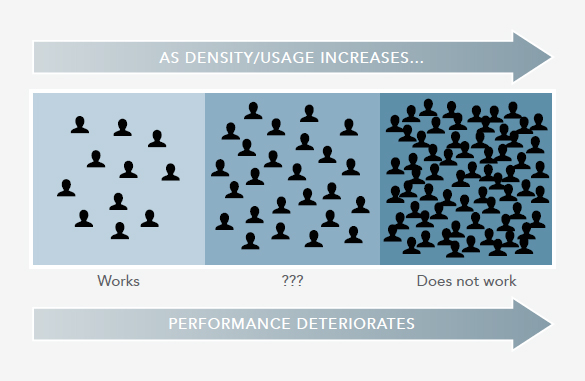
\includegraphics[width=9cm]{high-density-environments.jpg}
        \caption{Consequences of under-scoping wireless network design in high-density environments}
    \end{figure}
\end{frame}


\begin{frame}
	\frametitle{Problem}
	Potential approaches to address this issue are:\pause
	\begin{itemize}
		\item <2-> Deploy additional access points, though this increases cost and offers limited scalability;
		\item <3-> Employ multicast delivery, which conserves bandwidth but lacks reliability and content protection;
		\item <4-> Utilize device-to-device offloading to reduce access-point load and improve packet recovery;
		
	\end{itemize}
\end{frame}

\begin{frame}
	\frametitle{Problem: State of Art}
	
	\newcommand{\cmark}{\ding{52}}% Check mark
	\newcommand{\xmark}{\ding{55}}% Cross mark
	
	\centering
	\begin{tabular}{|l|c|c|c|}
		\hline
		\textbf{Work \& Reference} & \textbf{Adaptivity} & \textbf{Edge Offload} & \textbf{Security} \\
		\hline
		Real-time NC  & \xmark & \xmark & \xmark \\
		\hline
		AMuSe & Rate tuning & \xmark & \xmark \\
		\hline
		FlexFEC & Static/Matrix & \xmark & \xmark \\
		\hline
		RL-AFEC & Adaptive & \xmark & \xmark \\
		\hline
		Wi-Fi Direct & Heuristic & \textbf{\cmark} & App-dep. \\
		\hline
		IRIS & Predictive & \textbf{\cmark} & \textbf{\cmark} \\
		\hline
		Hyrax & Resource aware & \textbf{\cmark} & \xmark \\
		\hline
	\end{tabular}
	
	
\end{frame}


\begin{frame}
\frametitle{Introduction: Fog Computing}
   	\textbf{Fog Computing} refers to the process of extending cloud functions to nearby distributed nodes that sit close to end users, where these nodes perform local computation and data processing to reduce latency and bandwidth use while the distant cloud handles larger workloads.
 
    \begin{figure}
        \centering
        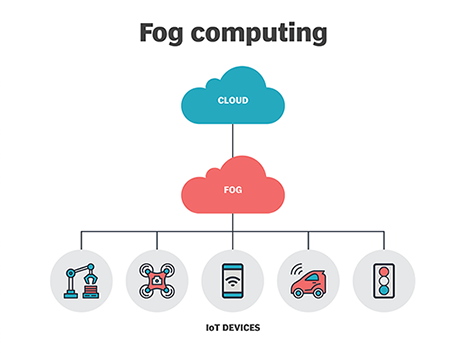
\includegraphics[width=7cm]{storage-fog_computing_mobile.png} 

    \end{figure}

\end{frame} 

\subsection{Goals}

\begin{frame}
\frametitle{Introduction: Goals}
    The main goals of this thesis are as follow:\pause
	\begin{itemize}
	   	\item <2-> \textbf{Design and Implement} a robust secure fog offloading prototype.
	   	\item <3-> \textbf{Develop} a custom network protocol to enable  integration of the offloading prototype.
	   	\item <4-> \textbf{Analyze and Validate} system performance, identifying key challenges and limitations.
	   	\item <5-> \textbf{Assess Viability} for broader adoption and deployment in high-density commercial environments.
	\end{itemize}
    
\end{frame}

\section{Architecture}

\subsection{Requirements}
\begin{frame}
	\frametitle{Architecture: Requirements}
	Based on the project's needs, the following requirements were devised:\pause
	\begin{itemize}
		\item <2-> Authentication \& Authorization
		\item <3-> Confidentiality \& Integrity
		\item <4-> Error Control
		\item <5-> Session Management
		\item <6-> Dynamic Path Selection
		\item <7-> Observability
		\item <8-> System Stability
	\end{itemize}
\end{frame}

\subsection{Architecture}

\begin{frame}
\frametitle{Architecture: Programming Language Choice}
    \begin{figure}
        \centering
        
\includegraphics[width=10cm]{Rust_vs_C.jpg}
        \caption{Rust vs C: Modern Safety Meets Classic Performance}
    \end{figure}
    
\end{frame}

\begin{frame}
\frametitle{Architecture: Overall System}

    \begin{figure}
        \centering
        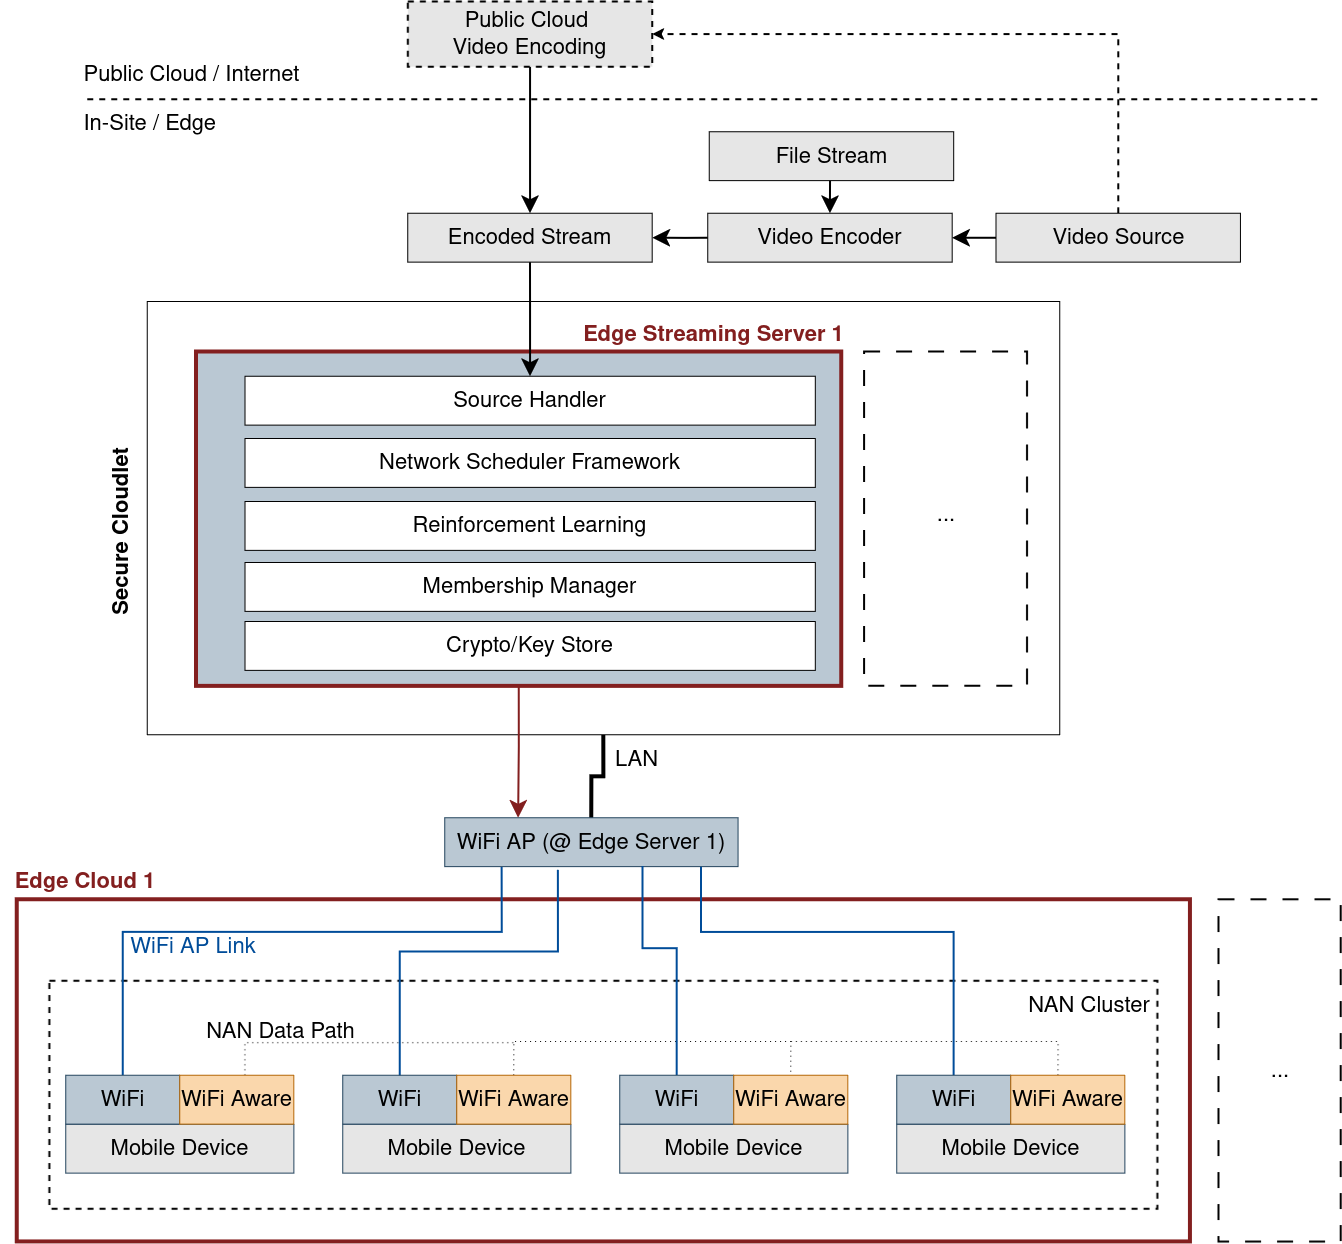
\includegraphics[width=8cm]{system.png}

    \end{figure}
\end{frame}

\subsection{Streaming Server}

\begin{frame}
\frametitle{Streaming Server: Source Stream Handler}
    \begin{itemize}
        \item <1-> Ingress Layer for Media Processing
        \item <2-> Storage of Buffered Data for Encoding
        \item <3-> Reed–Solomon Erasure Coding
    \end{itemize}
    \onslide<3>
    \begin{figure}
        \centering
        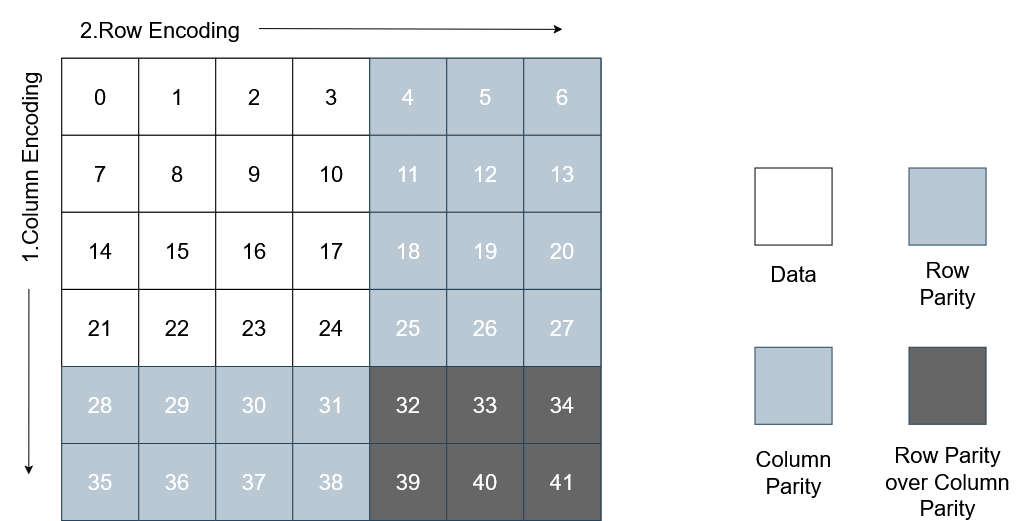
\includegraphics[width=10cm]{matrix_layout.png}
    \end{figure}
   
\end{frame}

\begin{frame}
	\frametitle{Streaming Server: Reinforcement Learning}
	\begin{figure}
		\centering
		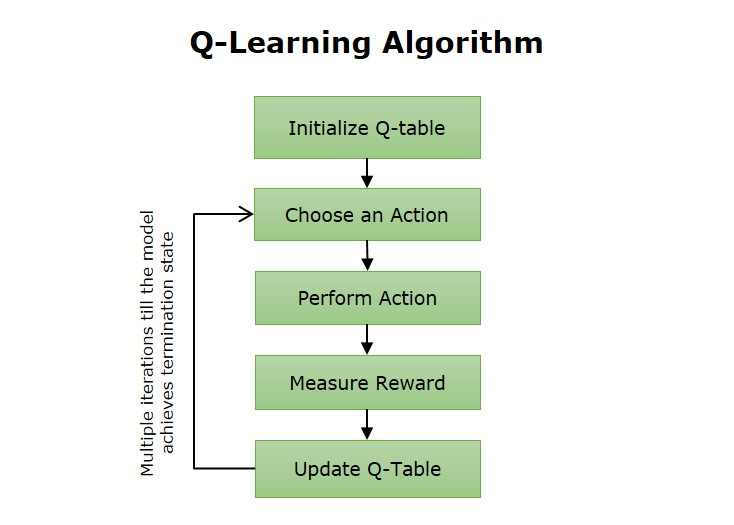
\includegraphics[width=10cm]{q_learning_algorithm.jpg}
	\end{figure}
	
\end{frame}


\begin{frame}
	\frametitle{Streaming Server: Reinforcement Learning}
	
	\textbf{Loss Classification}
	\[
	\text{loss\_bin}(x) =
	\begin{cases}
		0, & x < 1.0 \quad \text{(Excellent)} \\
		1, & 1.0 \leq x < 5.0 \quad \text{(Good)} \\
		2, & 5.0 \leq x < 10.0 \quad \text{(Moderate)} \\
		3, & 10.0 \leq x < 20.0 \quad \text{(Poor)} \\
		4, & x \geq 20.0 \quad \text{(Bad)}.
	\end{cases}
	\]
	
	\textbf{Reward Function}
	\[
	r(s,a) = -1.5 \cdot \text{loss\_bin}(s)
	- 10 \cdot \frac{\text{fec\_row}(a) + \text{fec\_col}(a)}
	{\text{data\_row} \cdot \text{data\_col}}.
	\]
	
\end{frame}

\begin{frame}
	\frametitle{Streaming Server: Membership Manager}
	
	
	\begin{itemize}
		\item <1-> Client Identification
		\item <2-> Efficient Feedback Handling
		\item <3-> Report Sink Processing
		\item <4-> Support for the Network Scheduler Framework
	\end{itemize}
	
	\onslide<4>
	\begin{figure}
		\centering
		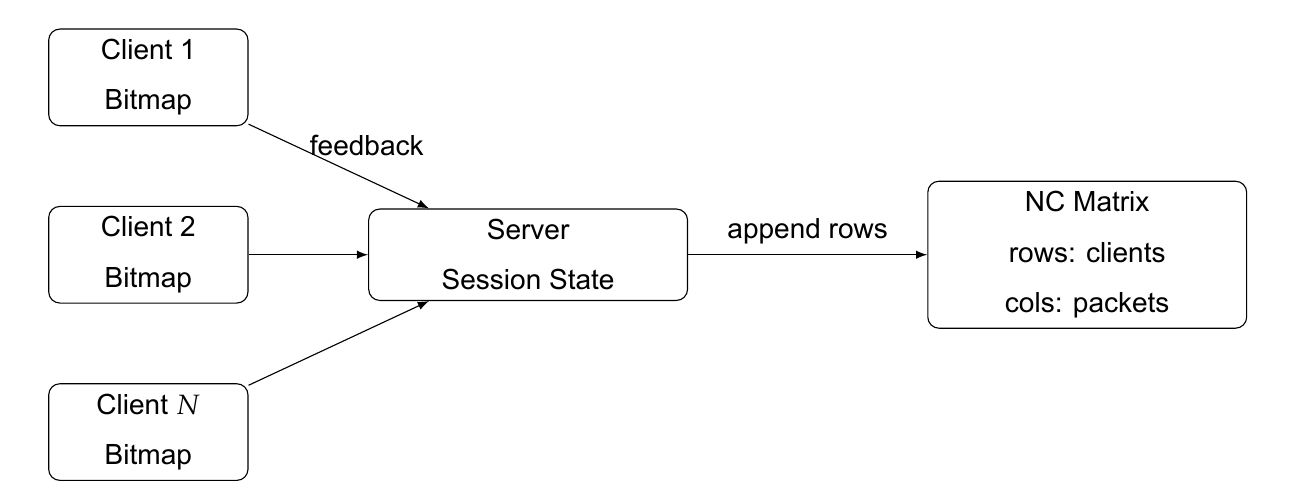
\includegraphics[width=10cm]{client_feedback.png}
	\end{figure}
	
\end{frame}

\begin{frame}
	\frametitle{Streaming Server: Network Scheduler Framework}
	\begin{itemize}
		\item <1-> Adaptive Multicast–Unicast Recovery
		\item <2-> Network Coding with NC Matrices
		\item <3-> Bandwidth-Aware Scheduling Loop
	\end{itemize}
	
	\onslide<3>
	\begin{figure}
		\centering
		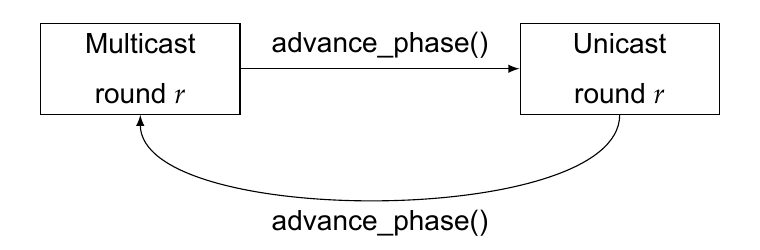
\includegraphics[width=10cm]{phase_advance.png}
	\end{figure}
	
\end{frame}

\begin{frame}
	\frametitle{Streaming Server: Network Scheduler Framework}
	
	\begin{figure}
		\centering
		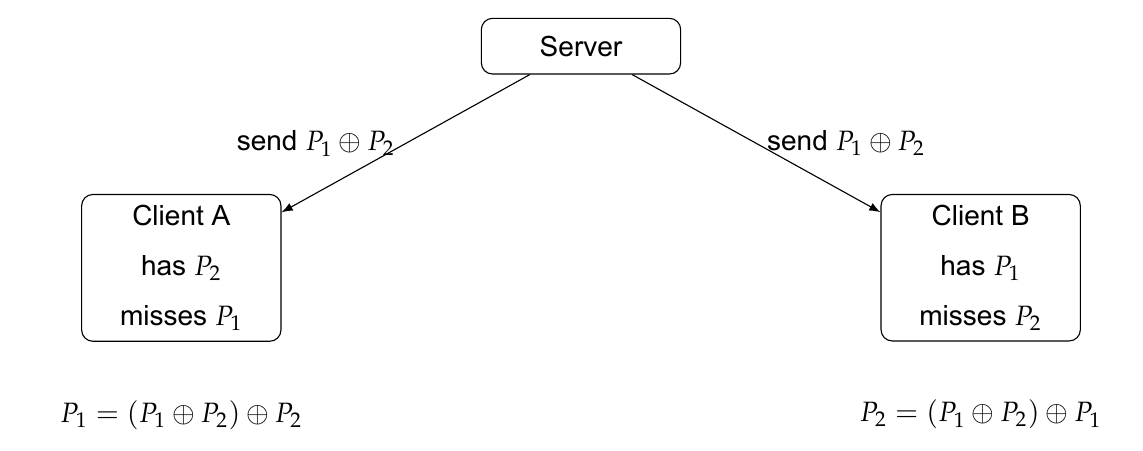
\includegraphics[width=12cm]{multicast_phase.png}
		\caption{A single coded multicast restores different packets at different receivers.}
	\end{figure}
	
\end{frame}


\subsection{Client Library}
\begin{frame}
	\frametitle{Client Library: Decoder}
	
	\begin{figure}
		\centering
		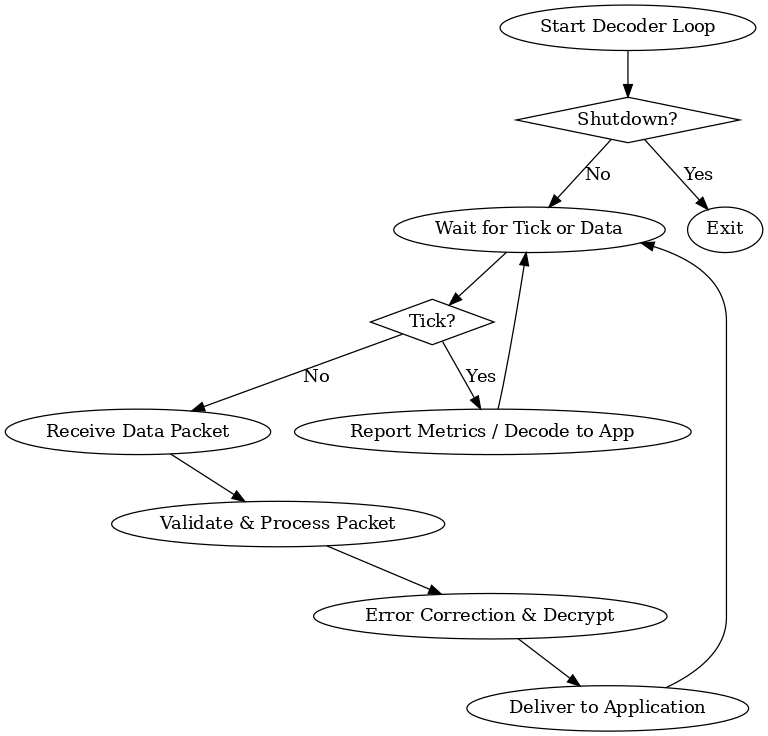
\includegraphics[width=7cm]{decoder_flowchart.png}
		\caption{Decoder Flowchart Diagram}
	\end{figure}
	
\end{frame}


\begin{frame}
	\frametitle{Client Library: Retransmission Manager}
	
	\begin{figure}
		\centering
		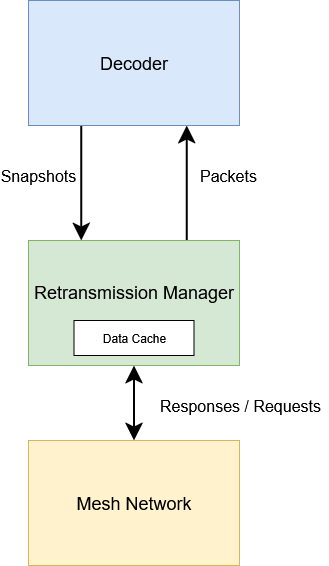
\includegraphics[width=4cm]{client_manager.png}

	\end{figure}
	
\end{frame}

\section{Mobile edge cloud offloading}

\begin{frame}
	\frametitle{Mobile edge cloud offloading: Wi-Fi Aware}
	
	\begin{figure}
		\centering
		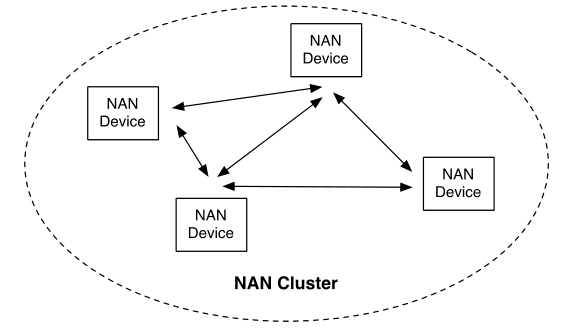
\includegraphics[width=10cm]{nan_cluster.png}
		\caption{NAN cluster topology, adapted from the Wi-Fi Aware Specification v4.0}
	\end{figure}
	
\end{frame}

\begin{frame}
	\frametitle{Mobile edge cloud offloading: Wi-Fi Aware}
	
	\begin{figure}
		\centering
		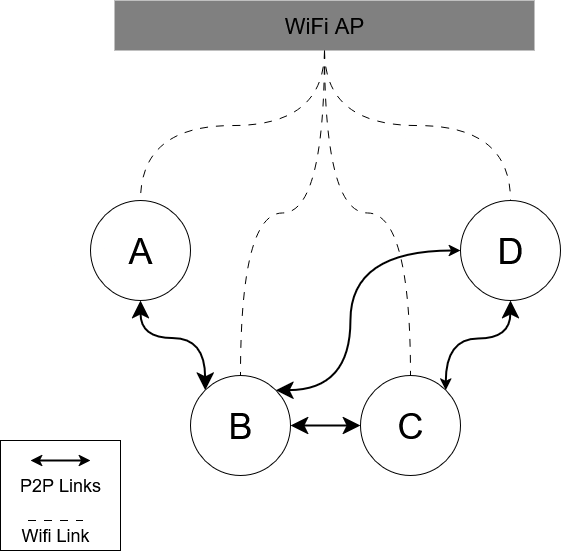
\includegraphics[width=7cm]{mesh_p2p.png}
	\end{figure}
	
\end{frame}

\begin{frame}
	\frametitle{Mobile edge cloud offloading: Mesh Networking}
	
	\begin{figure}
		\centering
		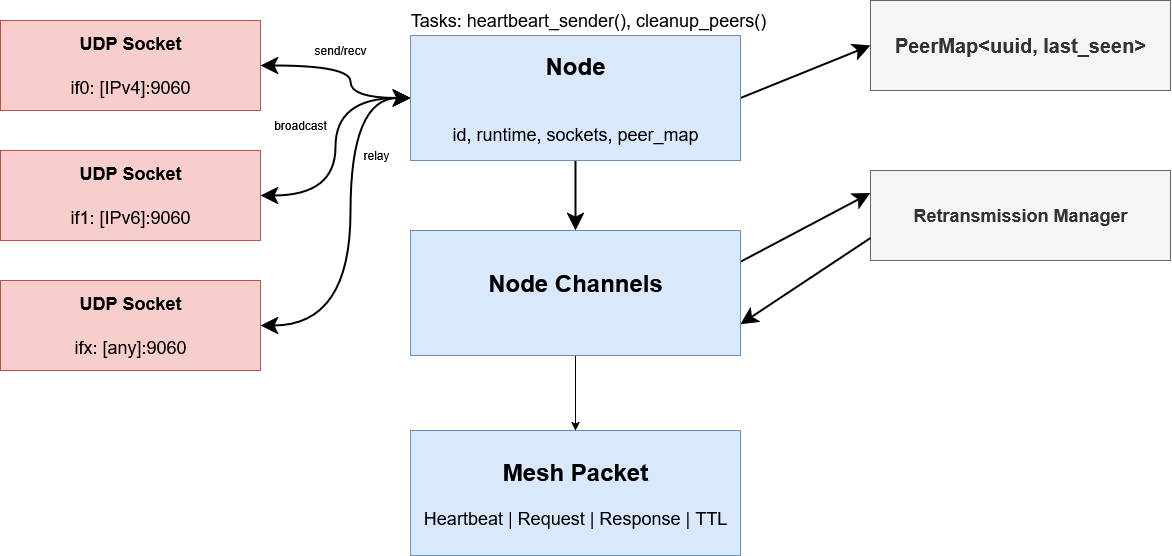
\includegraphics[width=11cm]{mesh_networking.png}
	\end{figure}
	
\end{frame}

\section{Frontend Implementation}

\begin{frame}
	\frametitle{Frontend Implementation: Android}
	
	\begin{figure}
		\centering
		\begin{minipage}[t]{.49\textwidth}
			\centering
			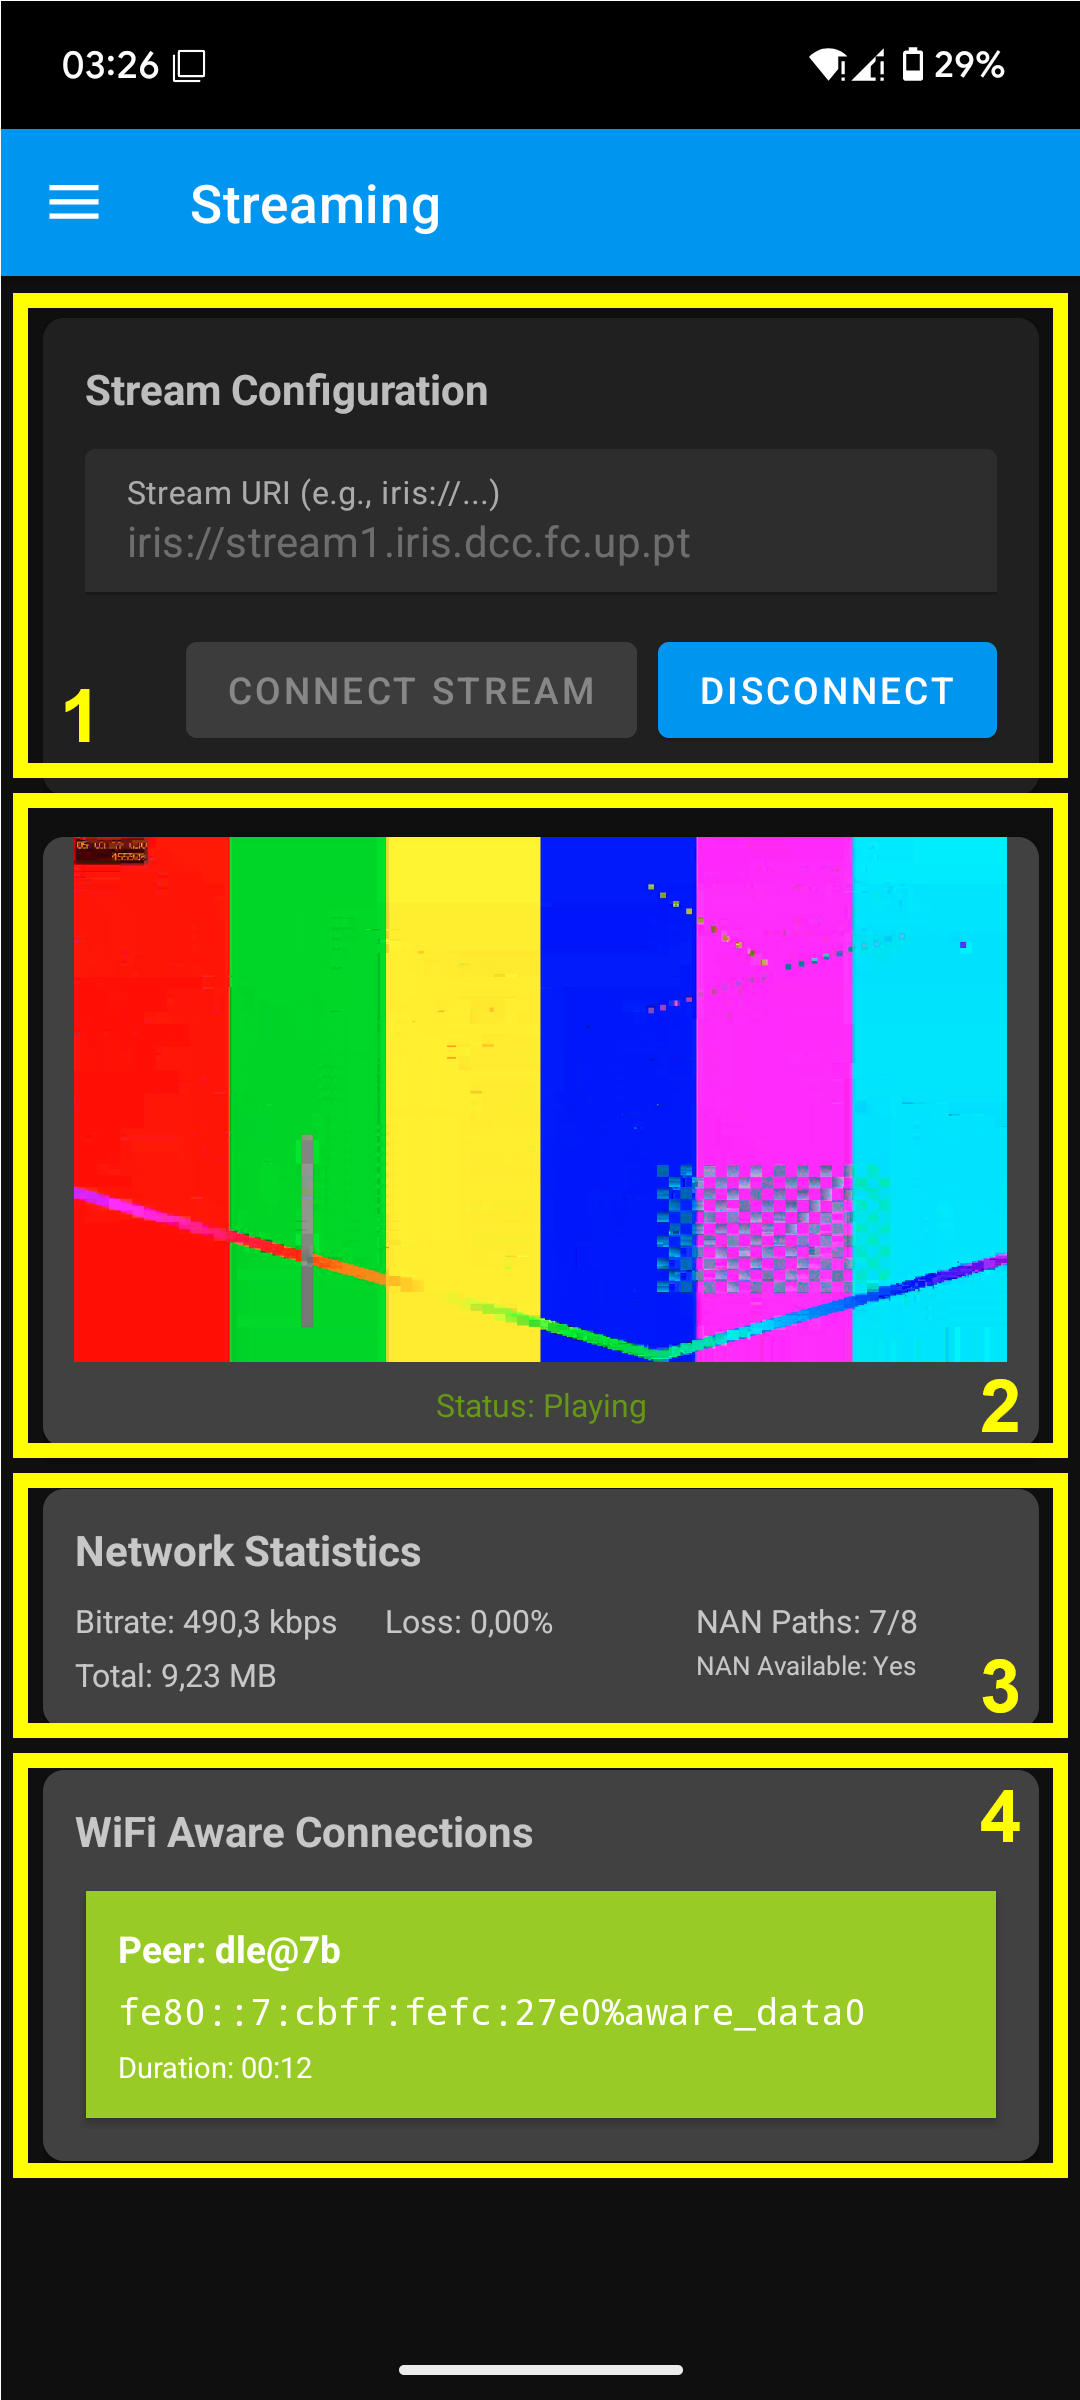
\includegraphics[height=0.8\textheight]{app_1.png}
			
		\end{minipage}%
		\hfill
		\begin{minipage}[t]{.49\textwidth}
			\centering
			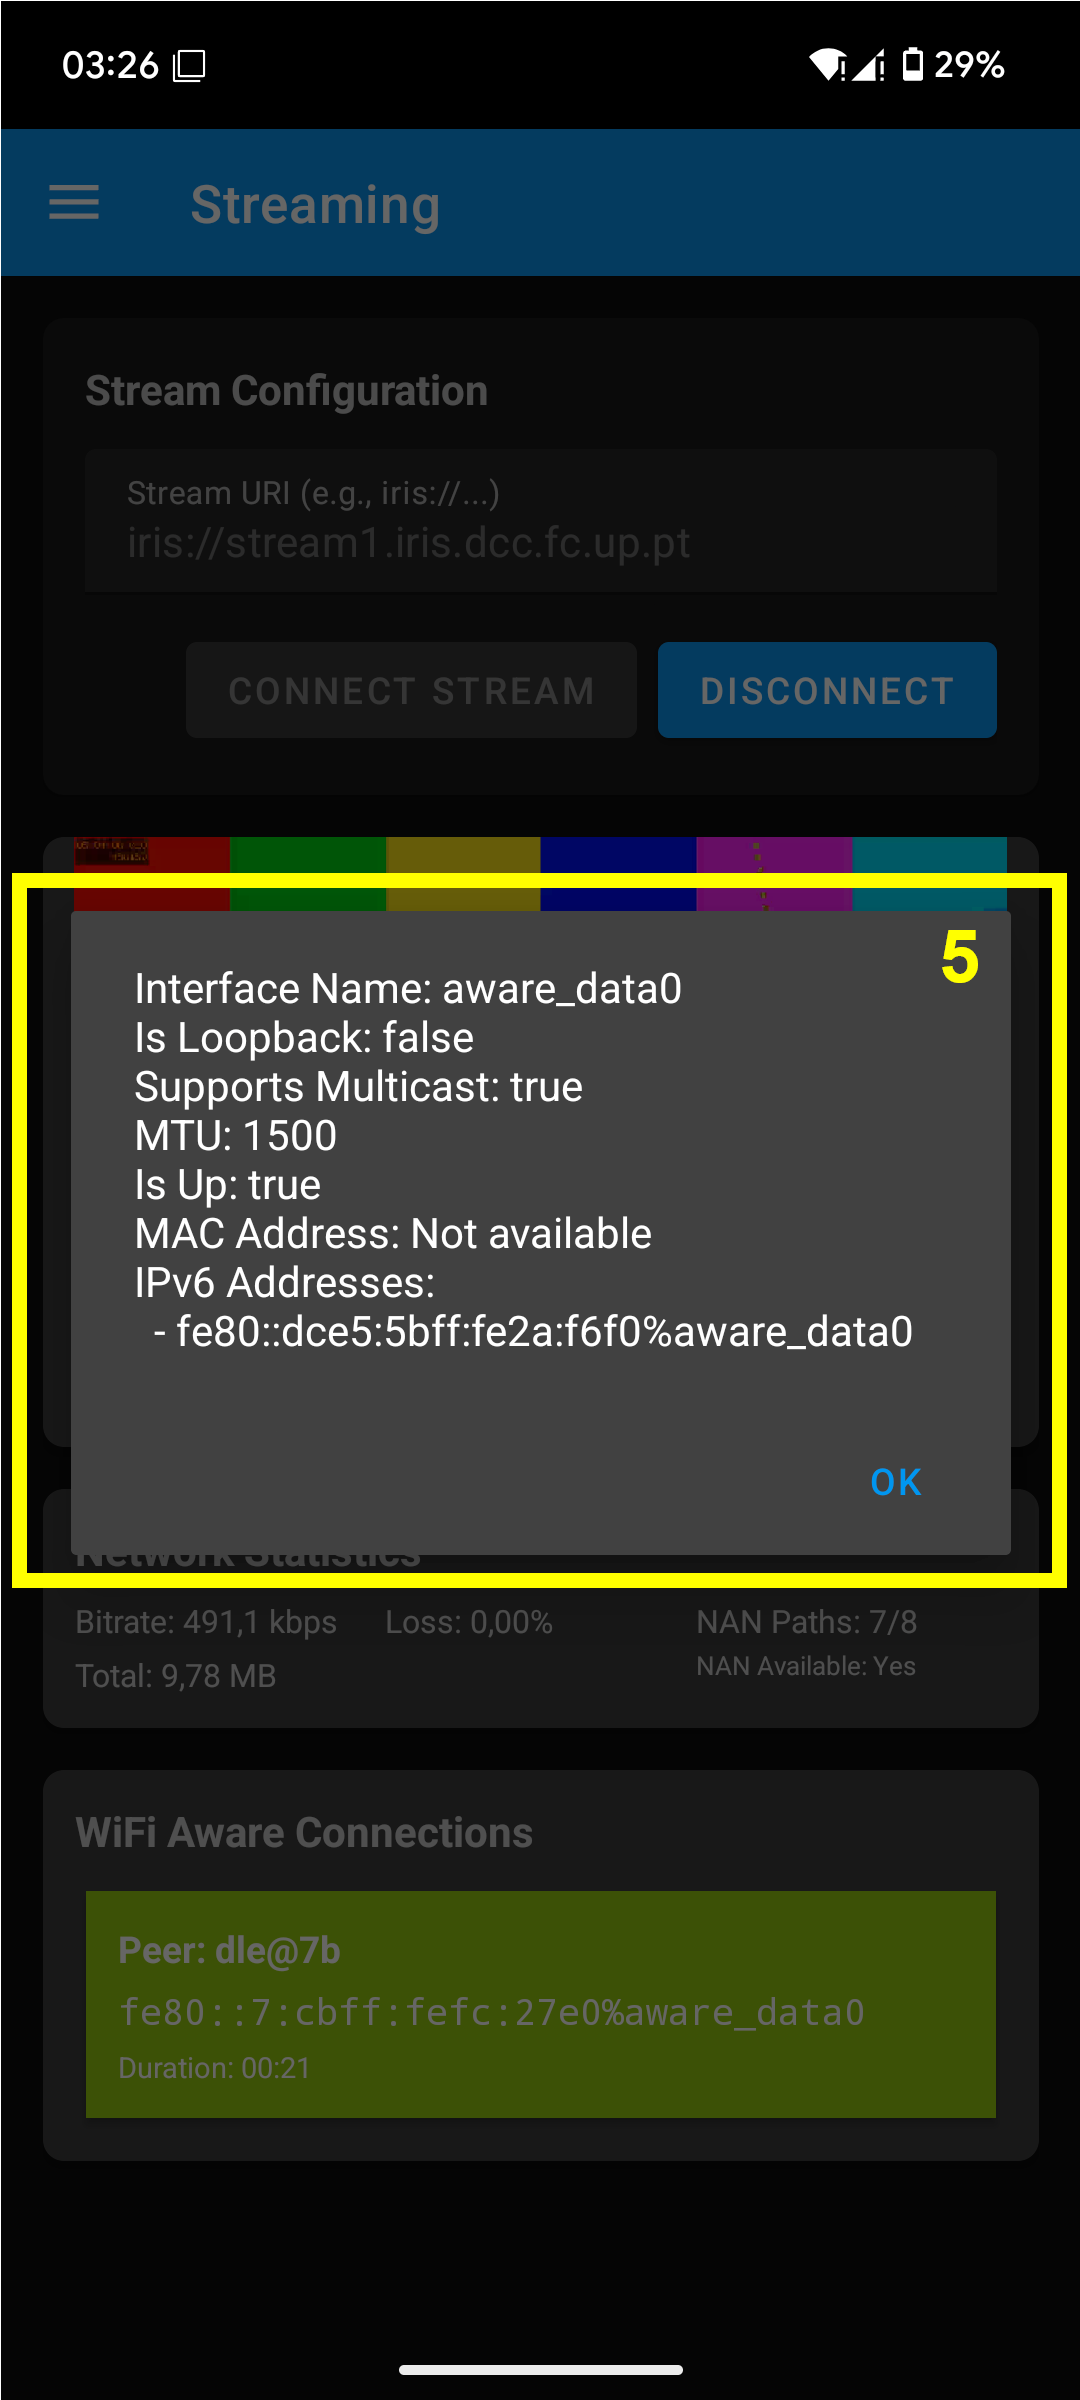
\includegraphics[height=0.8\textheight]{app_2.png}
			
		\end{minipage}
	\end{figure}
	
\end{frame}

\section{Security}

\begin{frame}
	\frametitle{Security}

	\begin{itemize}
		\item <1-> Authentication, Authorization, and Trust Model
		\item <2-> Forward Secrecy and Stream Integrity
		\item <3-> Double Signature Schema
	\end{itemize}
	
	\onslide<3>
	\begin{figure}
		\centering
		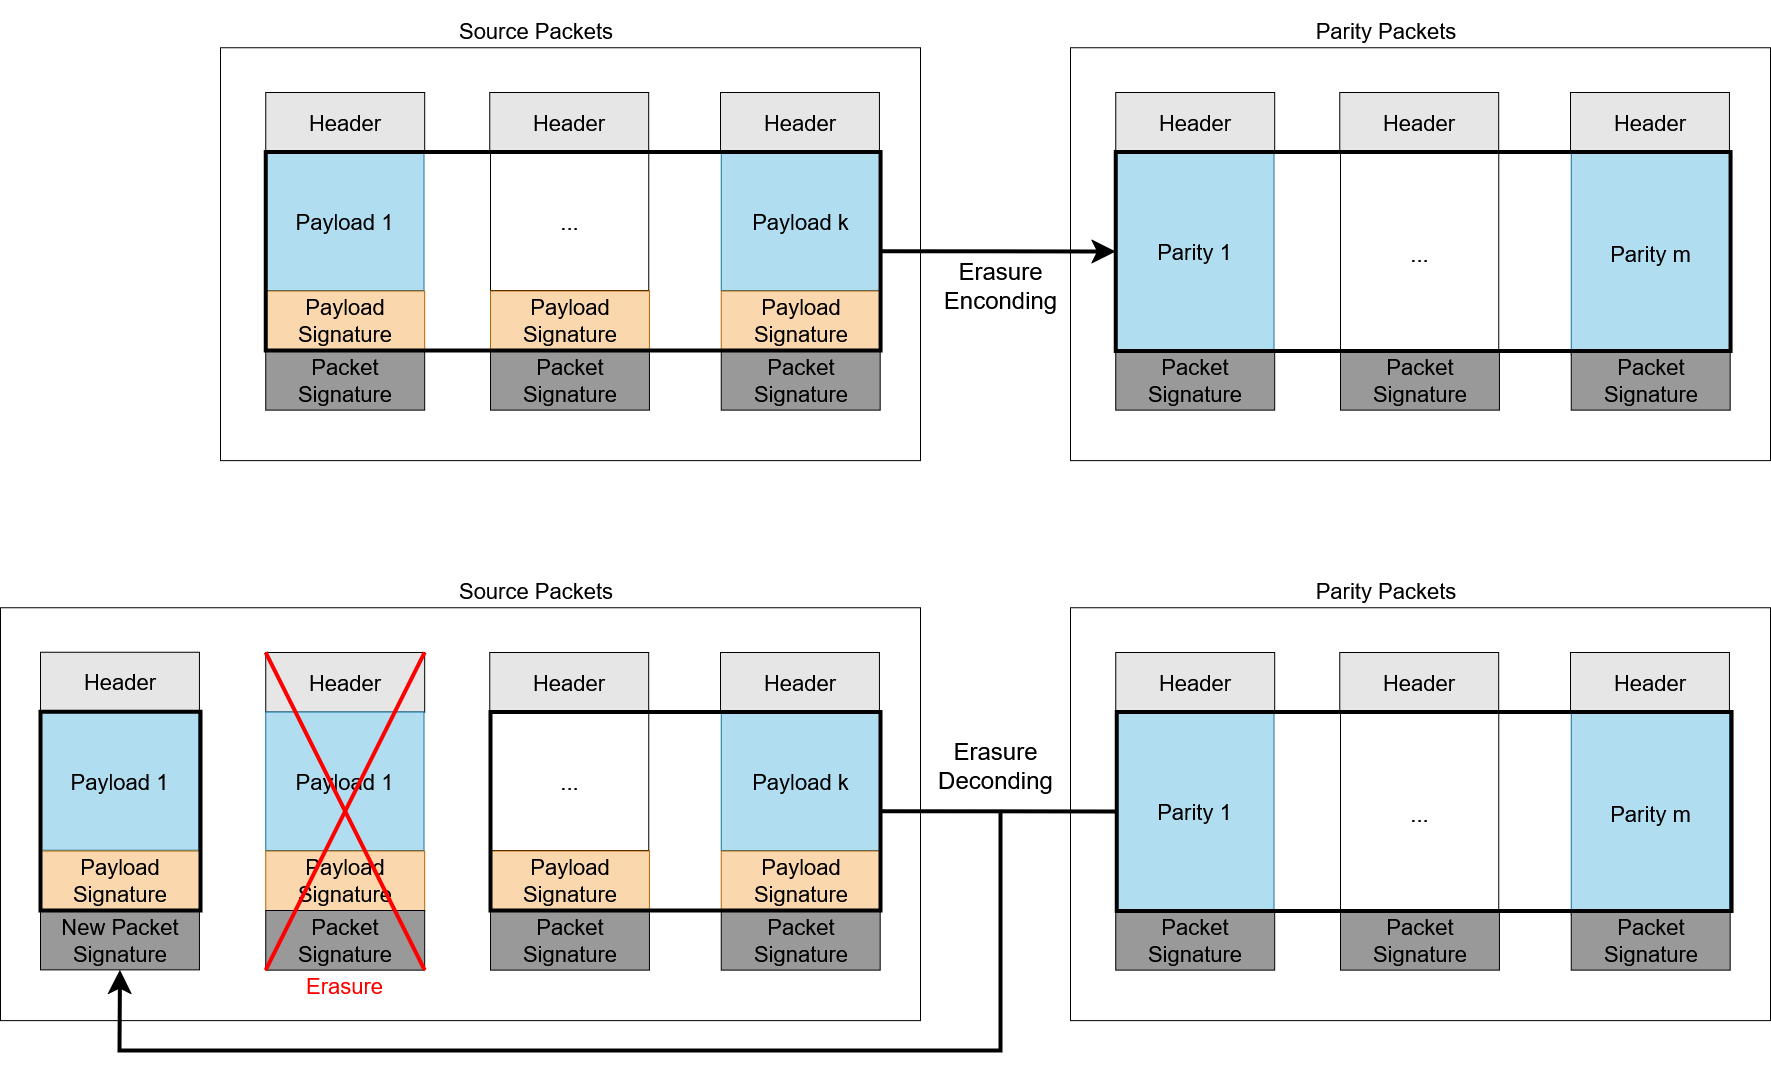
\includegraphics[width=10cm]{erasure_packet.png}
	\end{figure}
\end{frame}


\begin{frame}
	\frametitle{Security: Flow}
	
	\begin{figure}
		\centering
		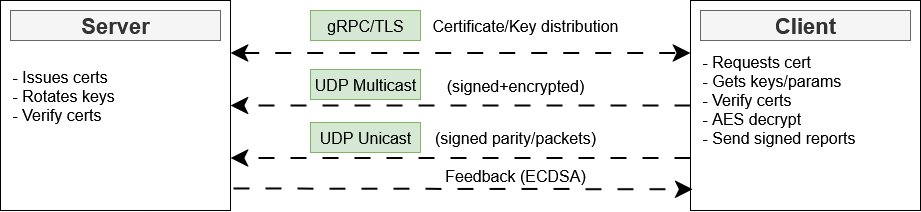
\includegraphics[width=11cm]{security_flow.png}
		\caption{Security flows between server and client}
	\end{figure}
\end{frame}

\section{Evaluation}    

\subsection{Environment}
\begin{frame}
	\frametitle{Evaluation: Environment}
	
	\begin{figure}
		\centering
		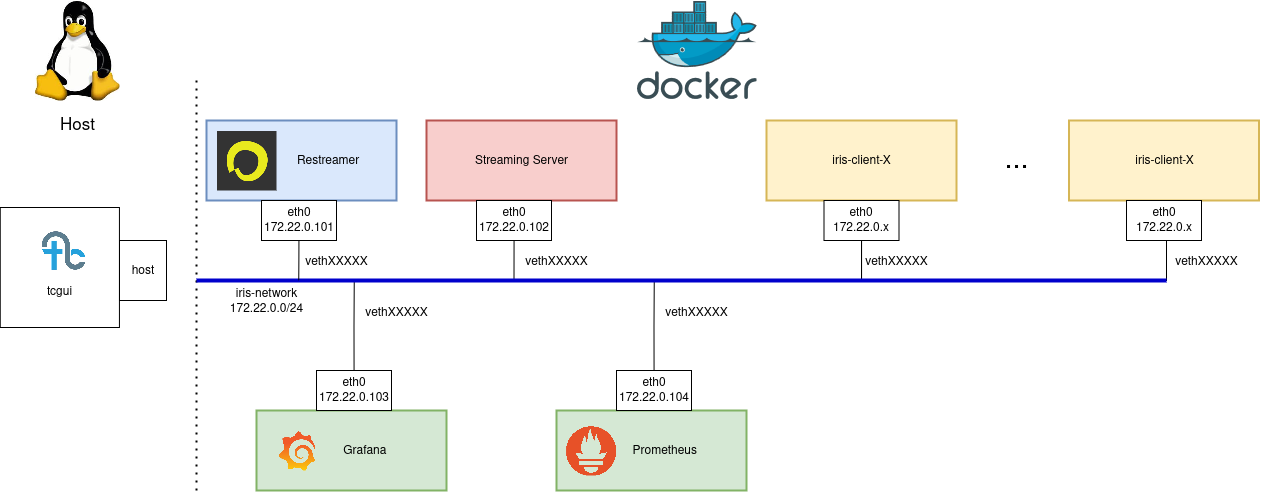
\includegraphics[width=11cm]{system_deployment.png}
		\caption{Containerized deployment of server, clients, and monitoring stack.}
	\end{figure}
\end{frame}

\subsection{Data Collection}
\begin{frame}
	\frametitle{Evaluation: Data Collection}
	
	\begin{figure}
		\centering
		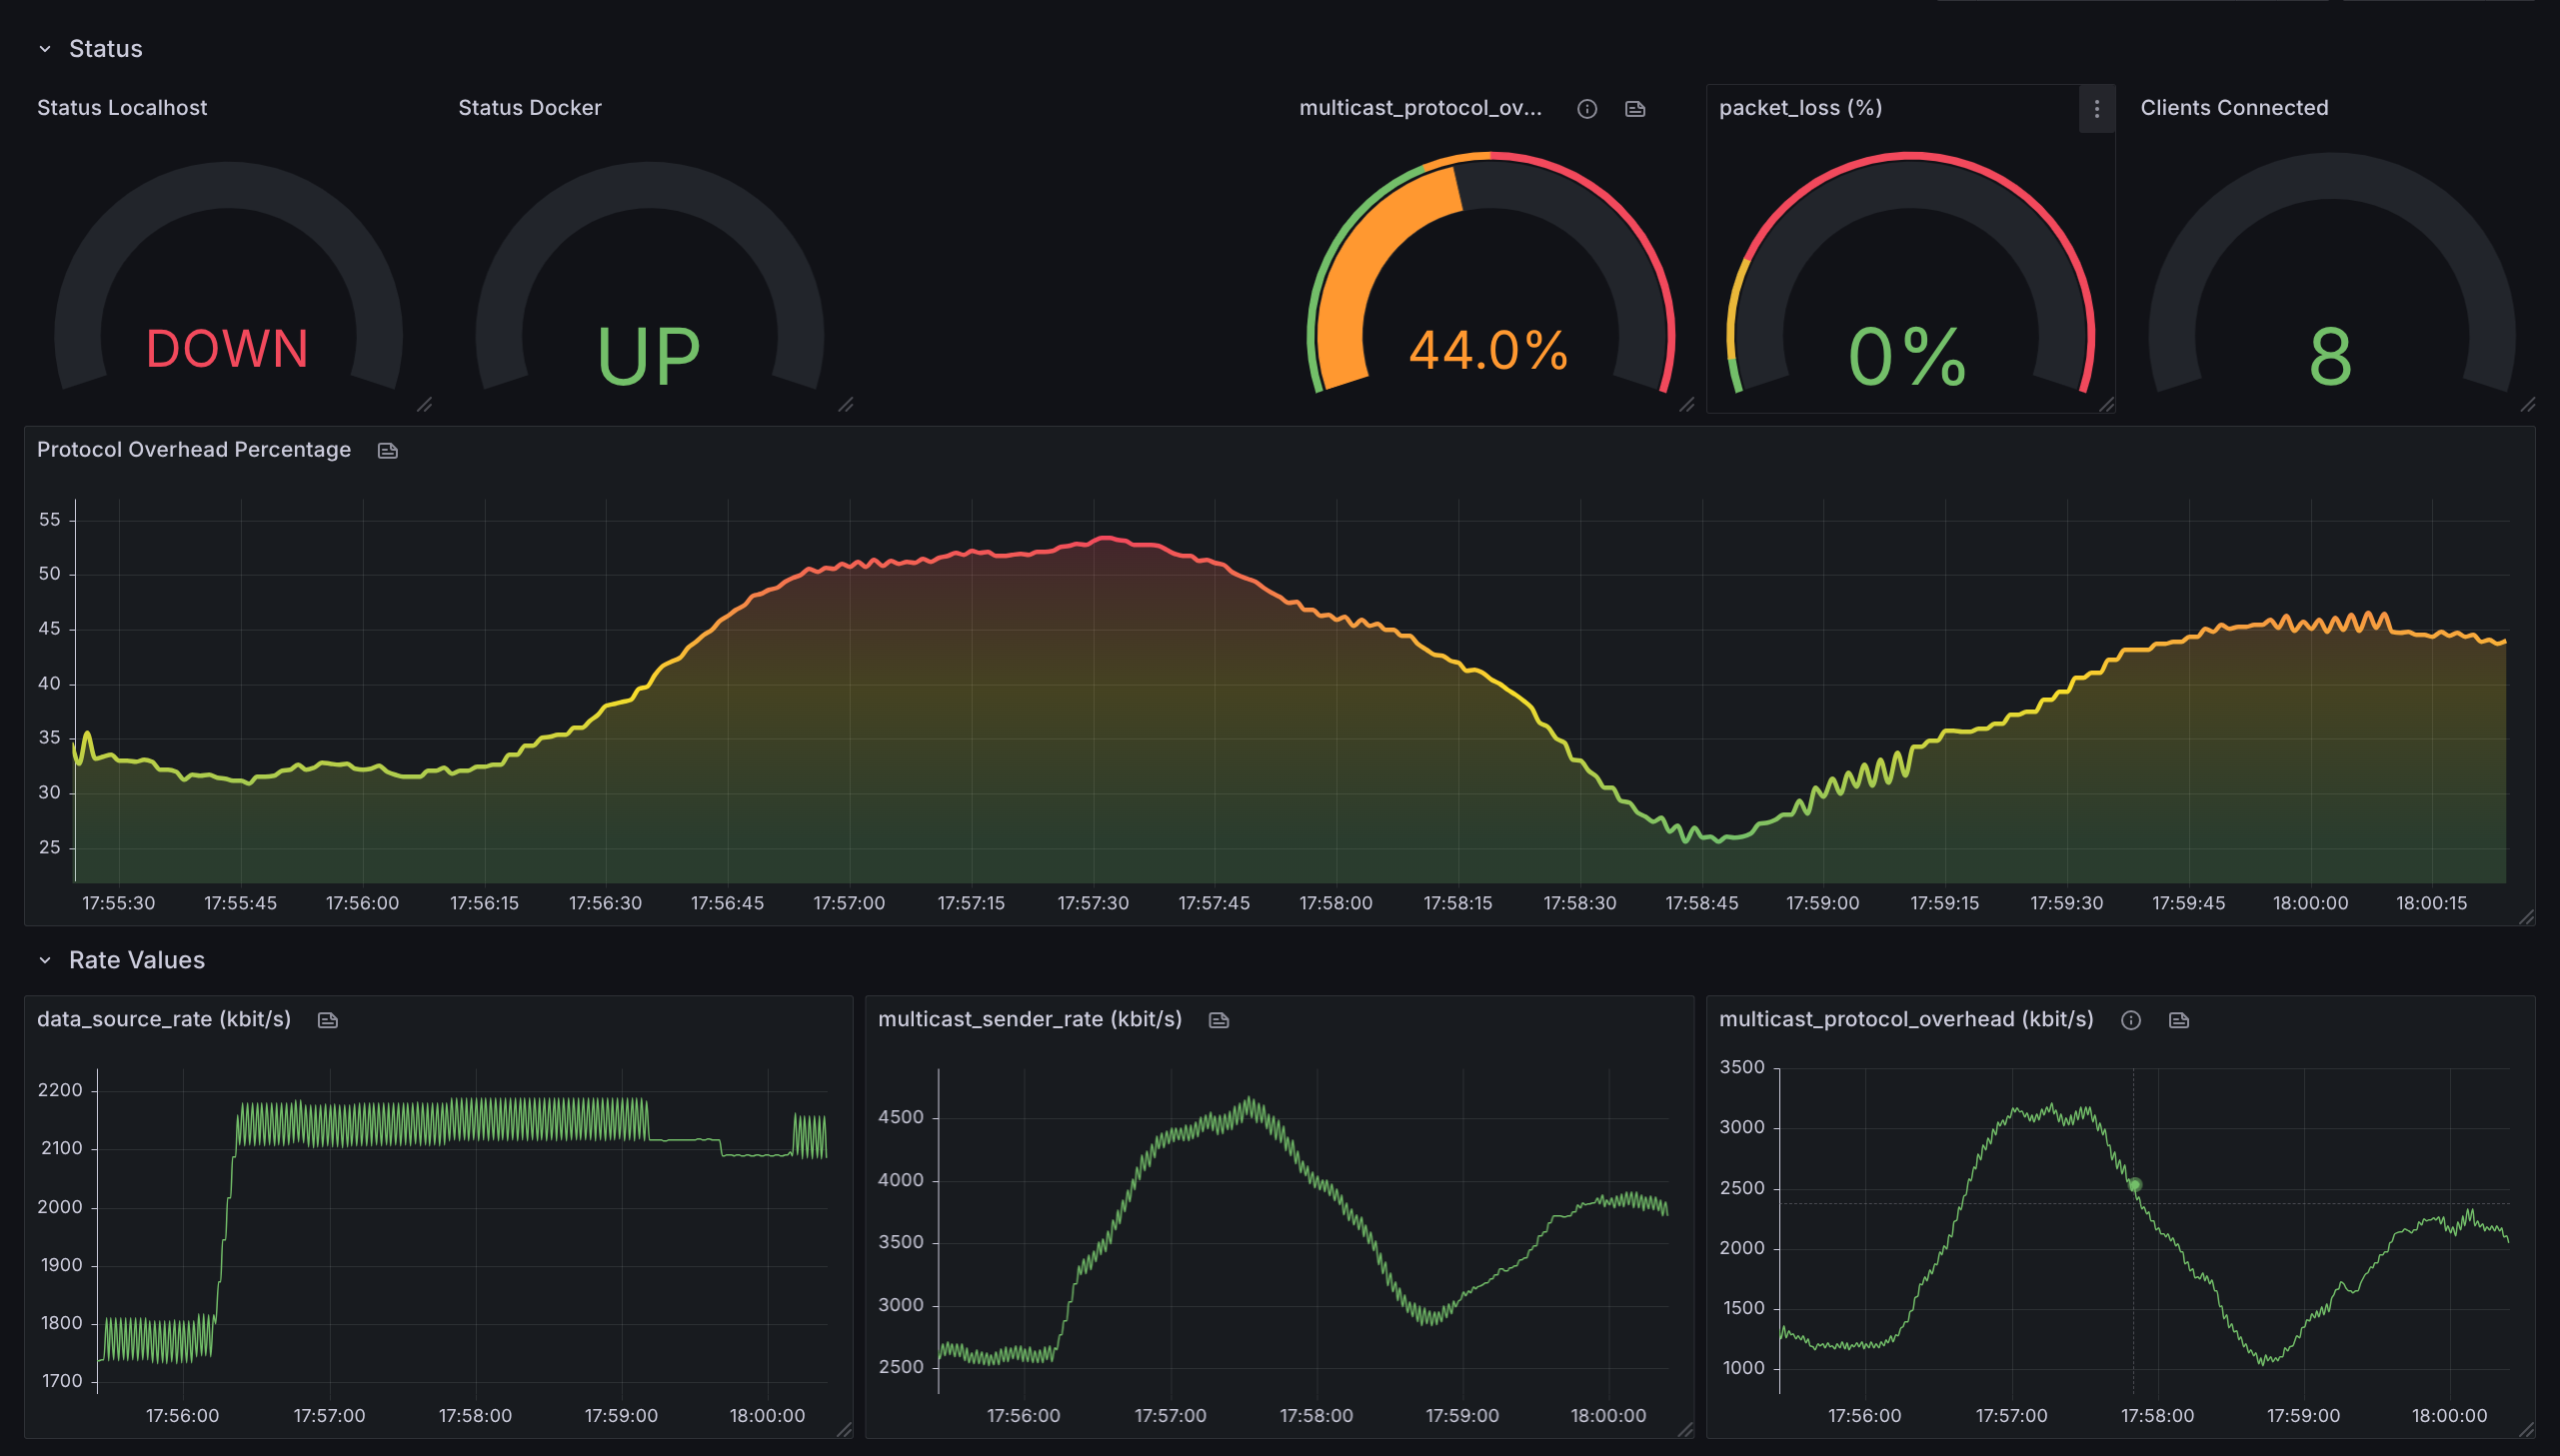
\includegraphics[width=12cm]{1.png}

	\end{figure}
\end{frame}

\begin{frame}
	\frametitle{Evaluation: Data Collection}
	
	\begin{figure}
		\centering
		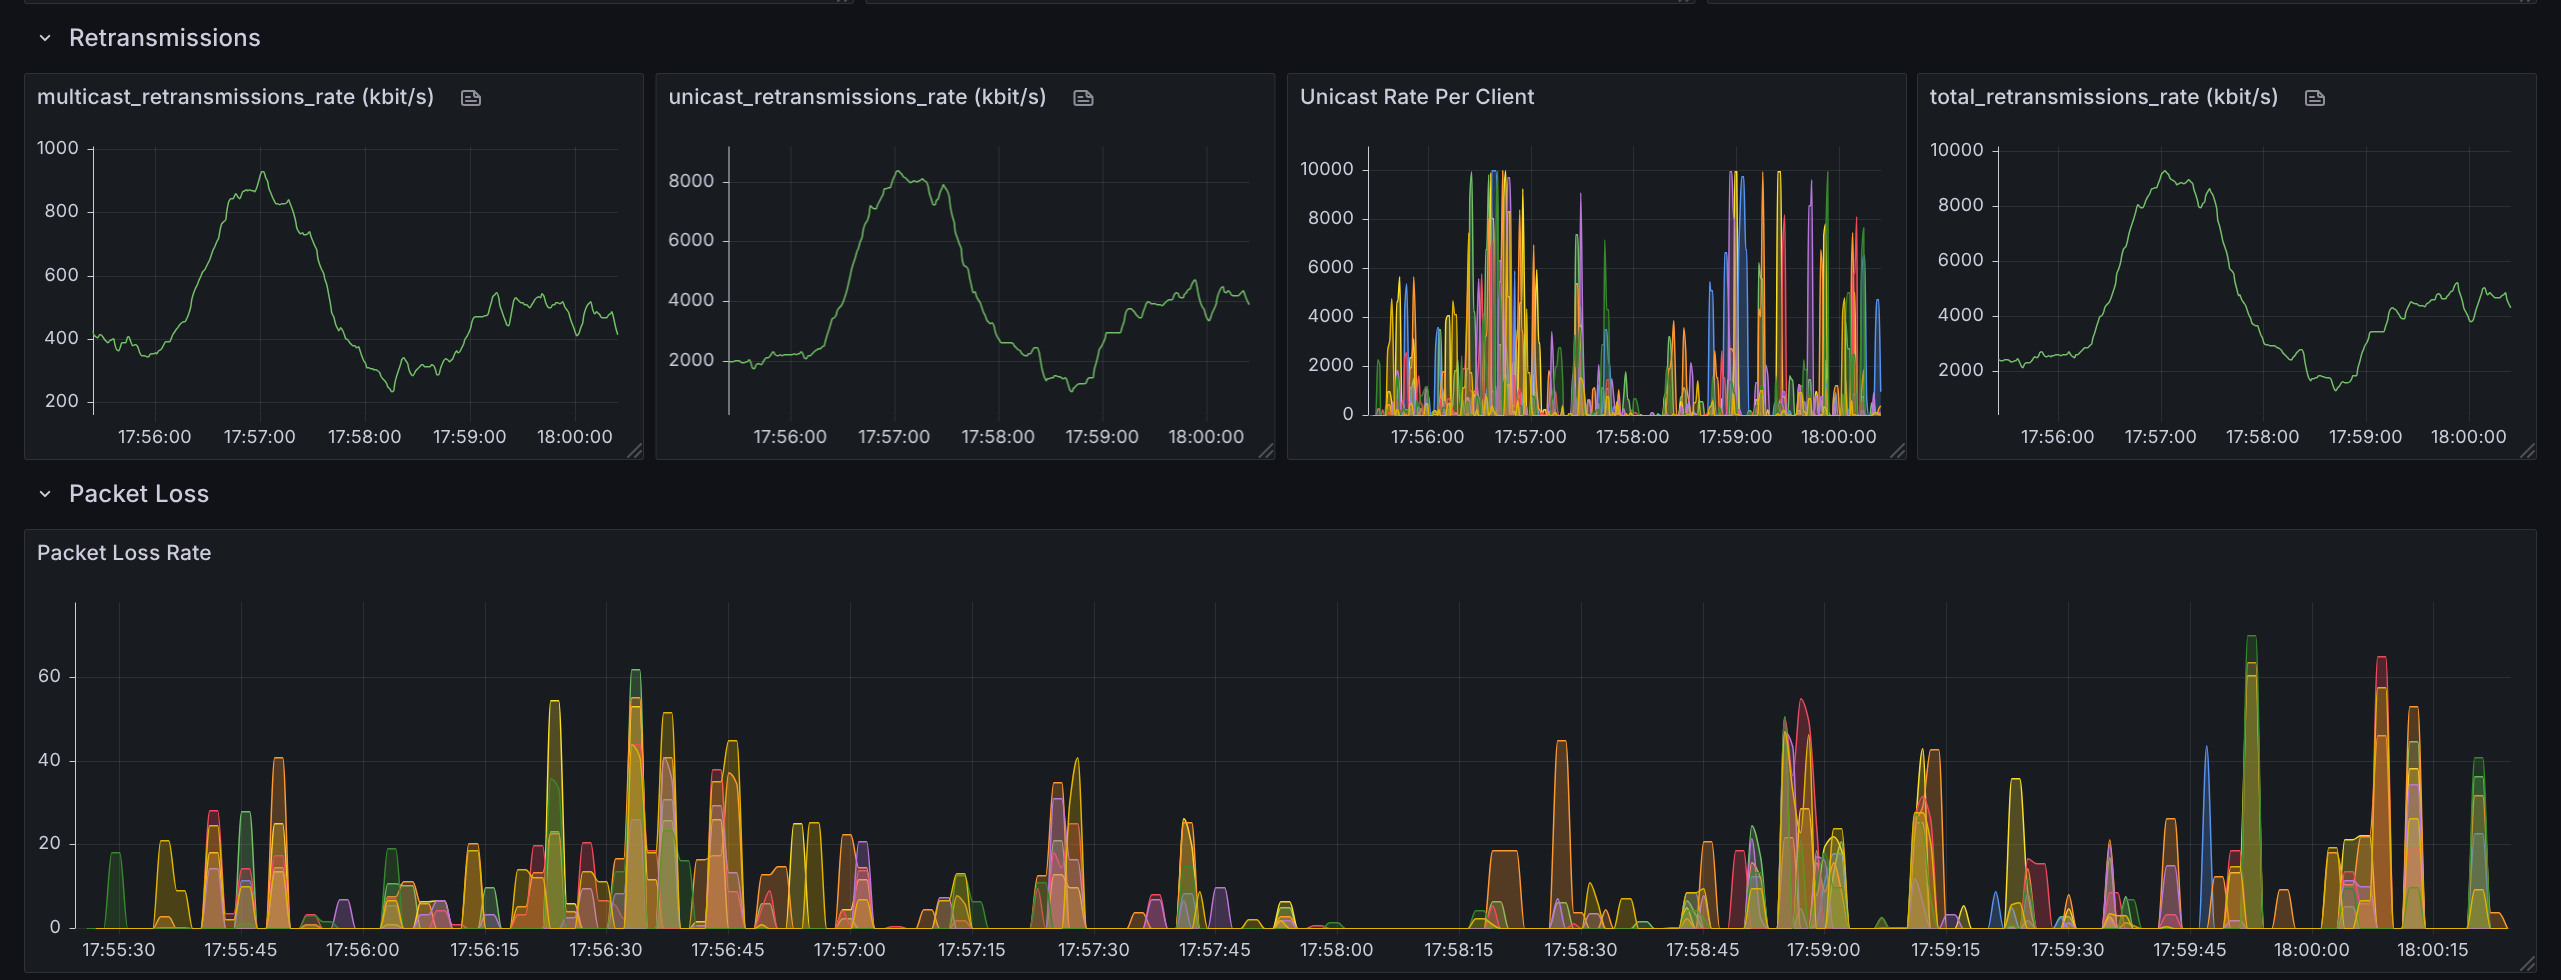
\includegraphics[width=12cm]{2.png}
		
	\end{figure}
\end{frame}

\begin{frame}
	\frametitle{Evaluation: Data Collection}
	
	\begin{figure}
		\centering
		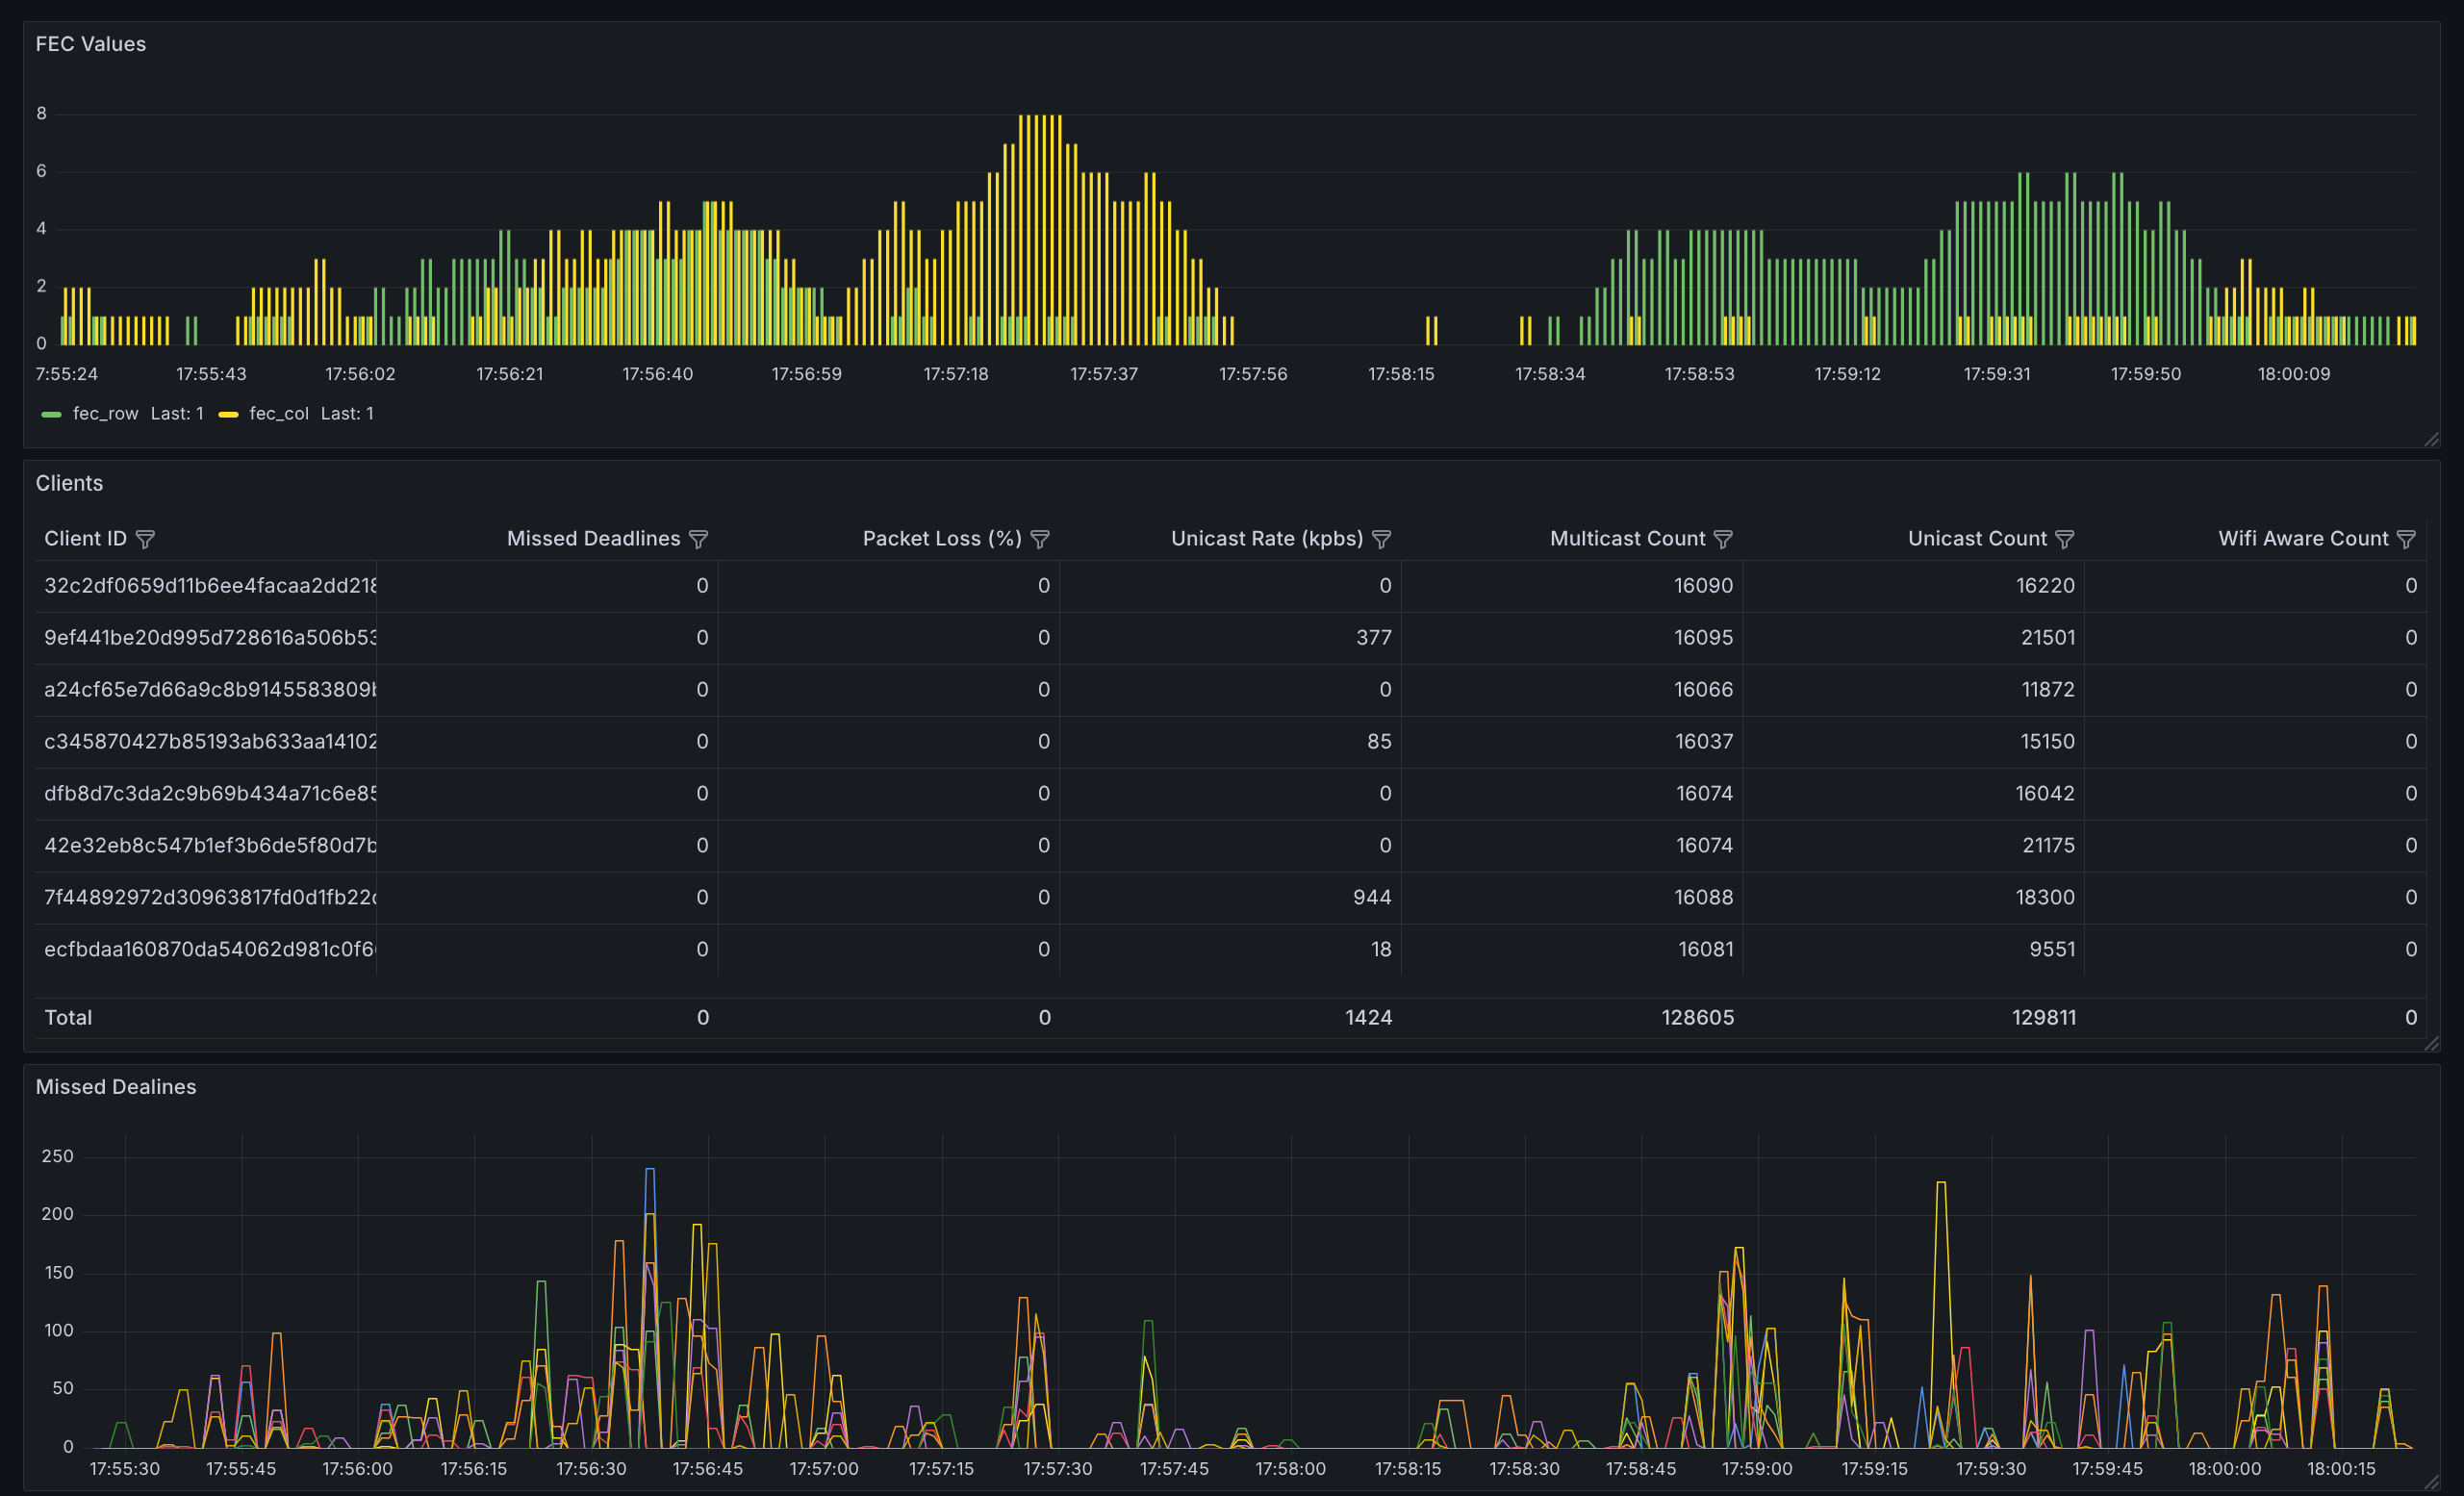
\includegraphics[width=12cm]{3.png}
		
	\end{figure}
\end{frame}

\begin{frame}
	\frametitle{Evaluation: Data Collection}
	
	\begin{figure}
		\centering
		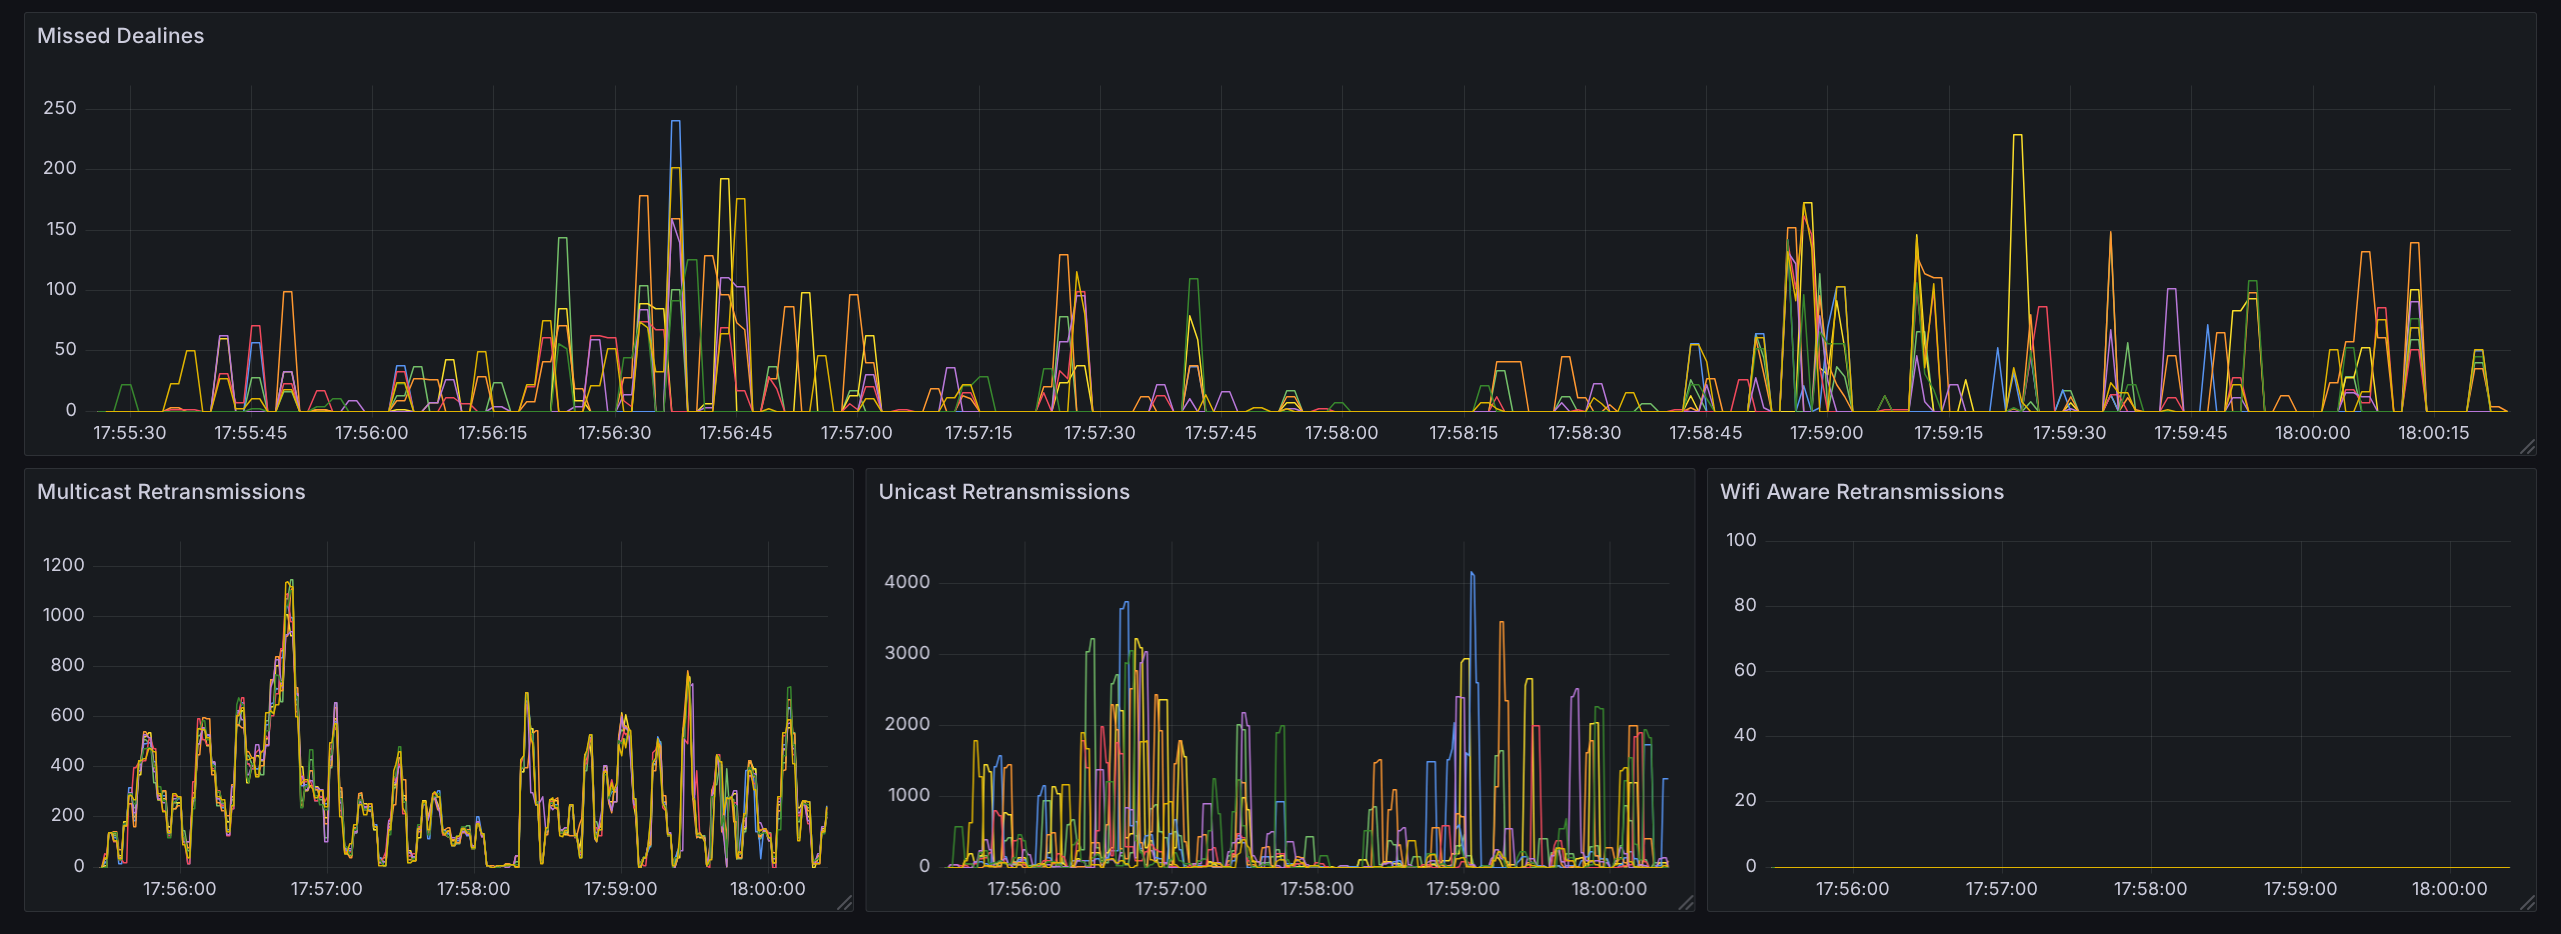
\includegraphics[width=12cm]{4.png}
		
	\end{figure}
\end{frame}


\subsection{Parameters}
\begin{frame}
	\frametitle{Evaluation: Parameters}
	
	\begin{table}
		\centering
		\begin{tabular}{lllll}
			\textbf{Scenario}             & \textbf{Retransmissions} & \textbf{FEC}    & \textbf{AI} & \textbf{Fog} \\
			\hline
			baseline                      & Off                      & None            & Off         & Off          \\
			ret\_on-fec\_off-ai\_off      & On                       & None            & Off         & Off          \\
		
			ret\_off-fec\_off-ai\_on      & Off                      & AI              & On          & Off          \\
			ret\_off-fec\_2x2-ai\_off     & Off                      & 2x2             & Off         & Off          \\
			ret\_off-fec\_1x1-ai\_off     & Off                      & 1x1             & Off         & Off          \\
			ret\_on-fec\_off-ai\_on       & On                       & AI              & On          & Off          \\
			ret\_on-fec\_2x2-ai\_off      & On                       & 2x2             & Off         & Off          \\
			Mobile\_baseline                  & Off                      & None            & Off         & Off          \\
			Mobile\_ret\_on-fog\_on           & On                       & None            & Off         & On           \\
			
		\end{tabular}
	
	\end{table}
\end{frame}

\subsection{Results}
\begin{frame}
	\frametitle{Evaluation: Results}
	
	\begin{itemize}
		\item <1-> \textbf{Static FEC performs poorly:} Increasing parity from 1x1 to 2x2 raised overhead from ~20\% to 44.7\% but did not reduce packet loss or missed deadlines. Fixed redundancy struggles when bursts hit multiple parities.
		\item <2-> T\textbf{argeted retransmission works best:} The scheduler cut average loss to 1.85\% and halved missed deadlines, keeping sender rate and overhead near baseline while focusing bandwidth on lost packets.
		
	\end{itemize}
\end{frame}

\begin{frame}
	\frametitle{Evaluation: Results}
	
	\begin{itemize}
		\item <1-> \textbf{Learning-driven FEC is inefficient:} Doubling sender rate and raising overhead to 57.5\% had little effect on reliability or deadlines. Extra redundancy wasted bandwidth.
		\item <2-> \textbf{Fog offloading reduces deadline misses:} Shifting recovery to nearby devices cut missed deadlines from 9464 to 1915 without increasing overhead, showing local recovery meets deadlines even with ongoing packet loss.
		
	\end{itemize}
\end{frame}


\section{Conclusion}
\begin{frame}
\frametitle{Conclusion}
    \begin{itemize}
    	\item \textbf{Findings:}
    	\begin{itemize}
    		\item Achieved reliable livestreaming.
    		\item Targeted retransmissions reduced missed deadlines.
    		\item Fog offloading decreased deadline misses.
    		\item Maintained security on untrusted fog nodes.
    	\end{itemize}
    	
    	\item \textbf{Limitations:}
    	\begin{itemize}
    		\item Static FEC proved inefficient, consuming high bandwidth.
    		\item Learning-driven FEC introduced excessive redundancy.
    		\item Real-world evaluations were limited to specific Wi-Fi conditions.
    		\item Wi-Fi Aware support is restricted to a limited set of devices.
    	\end{itemize}
    \end{itemize}
    
\end{frame}

\subsection{Contributions}
\begin{frame}
\frametitle{Conclusion}
        \textbf{Key Contributions:}
        \begin{itemize}
            \item Cross-platform runtime.
            \item Agnostic mesh implementation.
            \item Unified scheduler.
            \item Edge orchestration enables forwarding.
            \item Offloading via Wi-Fi Aware device-to-device communication.
        \end{itemize}
    % \end{itemize}
\end{frame}


\section{Future Work}
\begin{frame}
	\frametitle{Future Work}
	\begin{figure}
		\centering
		
\includegraphics[width=8cm]{libp2p.png}
		
	\end{figure}
\end{frame}

\end{document}
